\documentclass[]{standalone}
\usepackage{amsmath}
\usepackage{graphicx}
\usepackage[pdf]{pstricks}
\usepackage{pgfplots}
\pgfplotsset{compat=newest}
\usepgfplotslibrary{fillbetween}
%% the following commands are needed for some matlab2tikz features
\usetikzlibrary{plotmarks}
\usetikzlibrary{arrows.meta}
\usepgfplotslibrary{patchplots}
\usetikzlibrary{decorations.text}
\usetikzlibrary{shapes.multipart}


\definecolor{mycolor1}{rgb}{0.00000,0.44700,0.74100}%
\definecolor{mycolor2}{rgb}{0.85000,0.32500,0.09800}%
\definecolor{mycolor3}{rgb}{0.92900,0.69400,0.12500}%
\definecolor{mycolor4}{rgb}{0.49400,0.18400,0.55600}%
\definecolor{mycolor5}{rgb}{0.46600,0.67400,0.18800}%
\definecolor{mycolor6}{rgb}{0.30100,0.74500,0.93300}%
\definecolor{mycolor7}{rgb}{0.63500,0.07800,0.18400}%
%

\newcommand{\logLogSlopeTriangle}[5]
{
	% #1. Relative offset in x direction.
	% #2. Width in x direction, so xA-xB.
	% #3. Relative offset in y direction.
	% #4. Slope d(y)/d(log10(x)).
	% #5. Plot options.
	
	\pgfplotsextra
	{
		\pgfkeysgetvalue{/pgfplots/xmin}{\xmin}
		\pgfkeysgetvalue{/pgfplots/xmax}{\xmax}
		\pgfkeysgetvalue{/pgfplots/ymin}{\ymin}
		\pgfkeysgetvalue{/pgfplots/ymax}{\ymax}
		
		% Calculate auxilliary quantities, in relative sense.
		\pgfmathsetmacro{\xArel}{#1}
		\pgfmathsetmacro{\yArel}{#3}
		\pgfmathsetmacro{\xBrel}{#1-#2}
		\pgfmathsetmacro{\yBrel}{\yArel}
		\pgfmathsetmacro{\xCrel}{\xArel}
		%\pgfmathsetmacro{\yCrel}{ln(\yC/exp(\ymin))/ln(exp(\ymax)/exp(\ymin))} % REPLACE THIS EXPRESSION WITH AN EXPRESSION INDEPENDENT OF \yC TO PREVENT THE 'DIMENSION TOO LARGE' ERROR.
		
		\pgfmathsetmacro{\lnxB}{\xmin*(1-(#1-#2))+\xmax*(#1-#2)} % in [xmin,xmax].
		\pgfmathsetmacro{\lnxA}{\xmin*(1-#1)+\xmax*#1} % in [xmin,xmax].
		\pgfmathsetmacro{\lnyA}{\ymin*(1-#3)+\ymax*#3} % in [ymin,ymax].
		\pgfmathsetmacro{\lnyC}{\lnyA+#4*(\lnxA-\lnxB)}
		\pgfmathsetmacro{\yCrel}{\lnyC-\ymin)/(\ymax-\ymin)} % THE IMPROVED EXPRESSION WITHOUT 'DIMENSION TOO LARGE' ERROR.
		
		% Define coordinates for \draw. MIND THE 'rel axis cs' as opposed to the 'axis cs'.
		\coordinate (A) at (rel axis cs:\xArel,\yArel);
		\coordinate (B) at (rel axis cs:\xBrel,\yBrel);
		\coordinate (C) at (rel axis cs:\xCrel,\yCrel);
		
		% Draw slope triangle.
		\draw[#5]   (A)-- node[pos=0.5,anchor=north] {1}
		(B)-- 
		(C)-- node[pos=0.5,anchor=west] {#4}
		cycle;
	}
}

\begin{document}
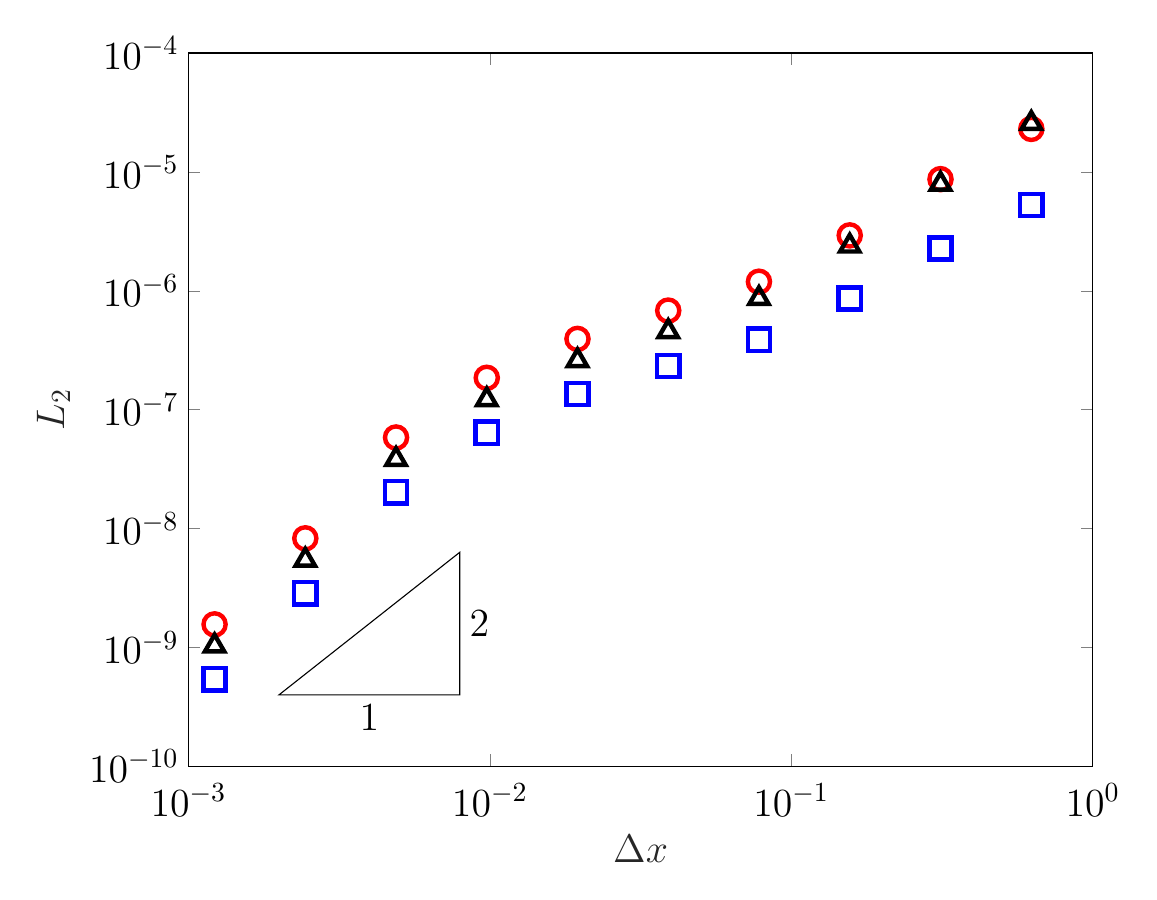
\begin{tikzpicture}
\tikzstyle{every node}=[font=\Large]
\begin{axis}[%
width=4.521in,
height=3.566in,
at={(0.758in,0.481in)},
scale only axis,
every axis plot/.append style={ultra thick},
xmode=log,
xmin=0.001,
xmax=1,
xtick={0.0001,  0.001,   0.01,    0.1,      1,     10},
xminorticks=false,
xlabel style={font=\color{white!15!black}},
xticklabel style = {yshift=-0.1cm},
xlabel={\Large $\Delta x$},
ymode=log,
ymin=1e-10,
ymax=0.0001,
ytick={ 1e-10,  1e-09,  1e-08,  1e-07,  1e-06,  1e-05, 0.0001},
yminorticks=false,
ylabel style={font=\color{white!15!black}},
ylabel={\Large $L_2$},
axis background/.style={fill=white}
]
 \logLogSlopeTriangle{0.3}{0.2}{0.1}{2}{black};

\addplot [color=blue, draw=none, mark=square, mark size=4pt, mark options={solid, blue}, forget plot]
  table[row sep=crcr]{%
5.05050505050505	0.000483698748844814\\
2.51256281407035	0.000169589965849294\\
1.2531328320802	3.32980538328303e-05\\
0.625782227784731	5.25590385193361e-06\\
0.312695434646654	2.26976104101581e-06\\
0.156298843388559	8.60577536699469e-07\\
0.0781372089388967	3.87423333098185e-07\\
0.0390655519962497	2.33758817007301e-07\\
0.0195320129692566	1.35716413772581e-07\\
0.00976581573858864	6.40350132918929e-08\\
0.00488286018418149	2.01644939575965e-08\\
0.00244141817098716	2.85539120856567e-09\\
0.00122070610523951	5.38621318202128e-10\\
};
\addplot [color=red, draw=none, mark=o, mark size=4pt, mark options={solid, red}, forget plot]
  table[row sep=crcr]{%
5.05050505050505	0.00115670707826559\\
2.51256281407035	0.000427477151877778\\
1.2531328320802	9.97462681343456e-05\\
0.625782227784731	2.30109580068174e-05\\
0.312695434646654	8.6929208427505e-06\\
0.156298843388559	2.92336444334387e-06\\
0.0781372089388967	1.19179652021004e-06\\
0.0390655519962497	6.81388961799862e-07\\
0.0195320129692566	3.93812876874036e-07\\
0.00976581573858864	1.85320441770844e-07\\
0.00488286018418149	5.83322647483121e-08\\
0.00244141817098716	8.27068640693104e-09\\
0.00122070610523951	1.56153240538376e-09\\
};
\addplot [color=black, draw=none, mark=triangle, mark size=4pt, mark options={solid, black}, forget plot]
  table[row sep=crcr]{%
5.05050505050505	0.00124826046863027\\
2.51256281407035	0.000368189887827043\\
1.2531328320802	9.79034675933332e-05\\
0.625782227784731	2.56447077484835e-05\\
0.312695434646654	7.90969355153622e-06\\
0.156298843388559	2.38368912558142e-06\\
0.0781372089388967	8.62559806532319e-07\\
0.0390655519962497	4.54440201860214e-07\\
0.0195320129692566	2.58867285076313e-07\\
0.00976581573858864	1.21399607437539e-07\\
0.00488286018418149	3.81974842642003e-08\\
0.00244141817098716	5.42957981678207e-09\\
0.00122070610523951	1.03140272416875e-09\\
};
\end{axis}
\end{tikzpicture}%
\end{document}